%Este trabalho está licenciado sob a Licença Creative Commons Atribuição-CompartilhaIgual 3.0 Não Adaptada. Para ver uma cópia desta licença, visite https://creativecommons.org/licenses/by-sa/3.0/ ou envie uma carta para Creative Commons, PO Box 1866, Mountain View, CA 94042, USA.

%\documentclass[main.tex]{subfiles}
%\begin{document}

\chapter{Interpolação}\index{aproximação!de funções}\label{cap:interp}

Neste capítulo, discutimos os problemas de \emph{interpolação}\index{interpolação}. Mais precisamente, dada uma sequência de $n$ reais $x_1<x_2<\ldots<x_n$, um conjunto de pontos $\left\{(x_i, y_i)\in I\times\mathbb{R}\right\}_{i=1}^n$, onde $I=\left[x_1,x_n\right]$ e uma família de funções $\mathcal{F}_I = \{\varphi:I\rightarrow\mathbb{R}\}$, o problema de interpolação consiste em encontrar alguma função $f\in\mathcal{F}_I$ tal que
\begin{equation}
  f(x_i) = y_i,\quad i=1, 2, \dotsc, n.
\end{equation}
Chamamos uma tal $f$ de \emph{função interpoladora} dos pontos dados. Ou ainda, dizemos que $f$ interpola os pontos dados.

\begin{figure}
  \centering
  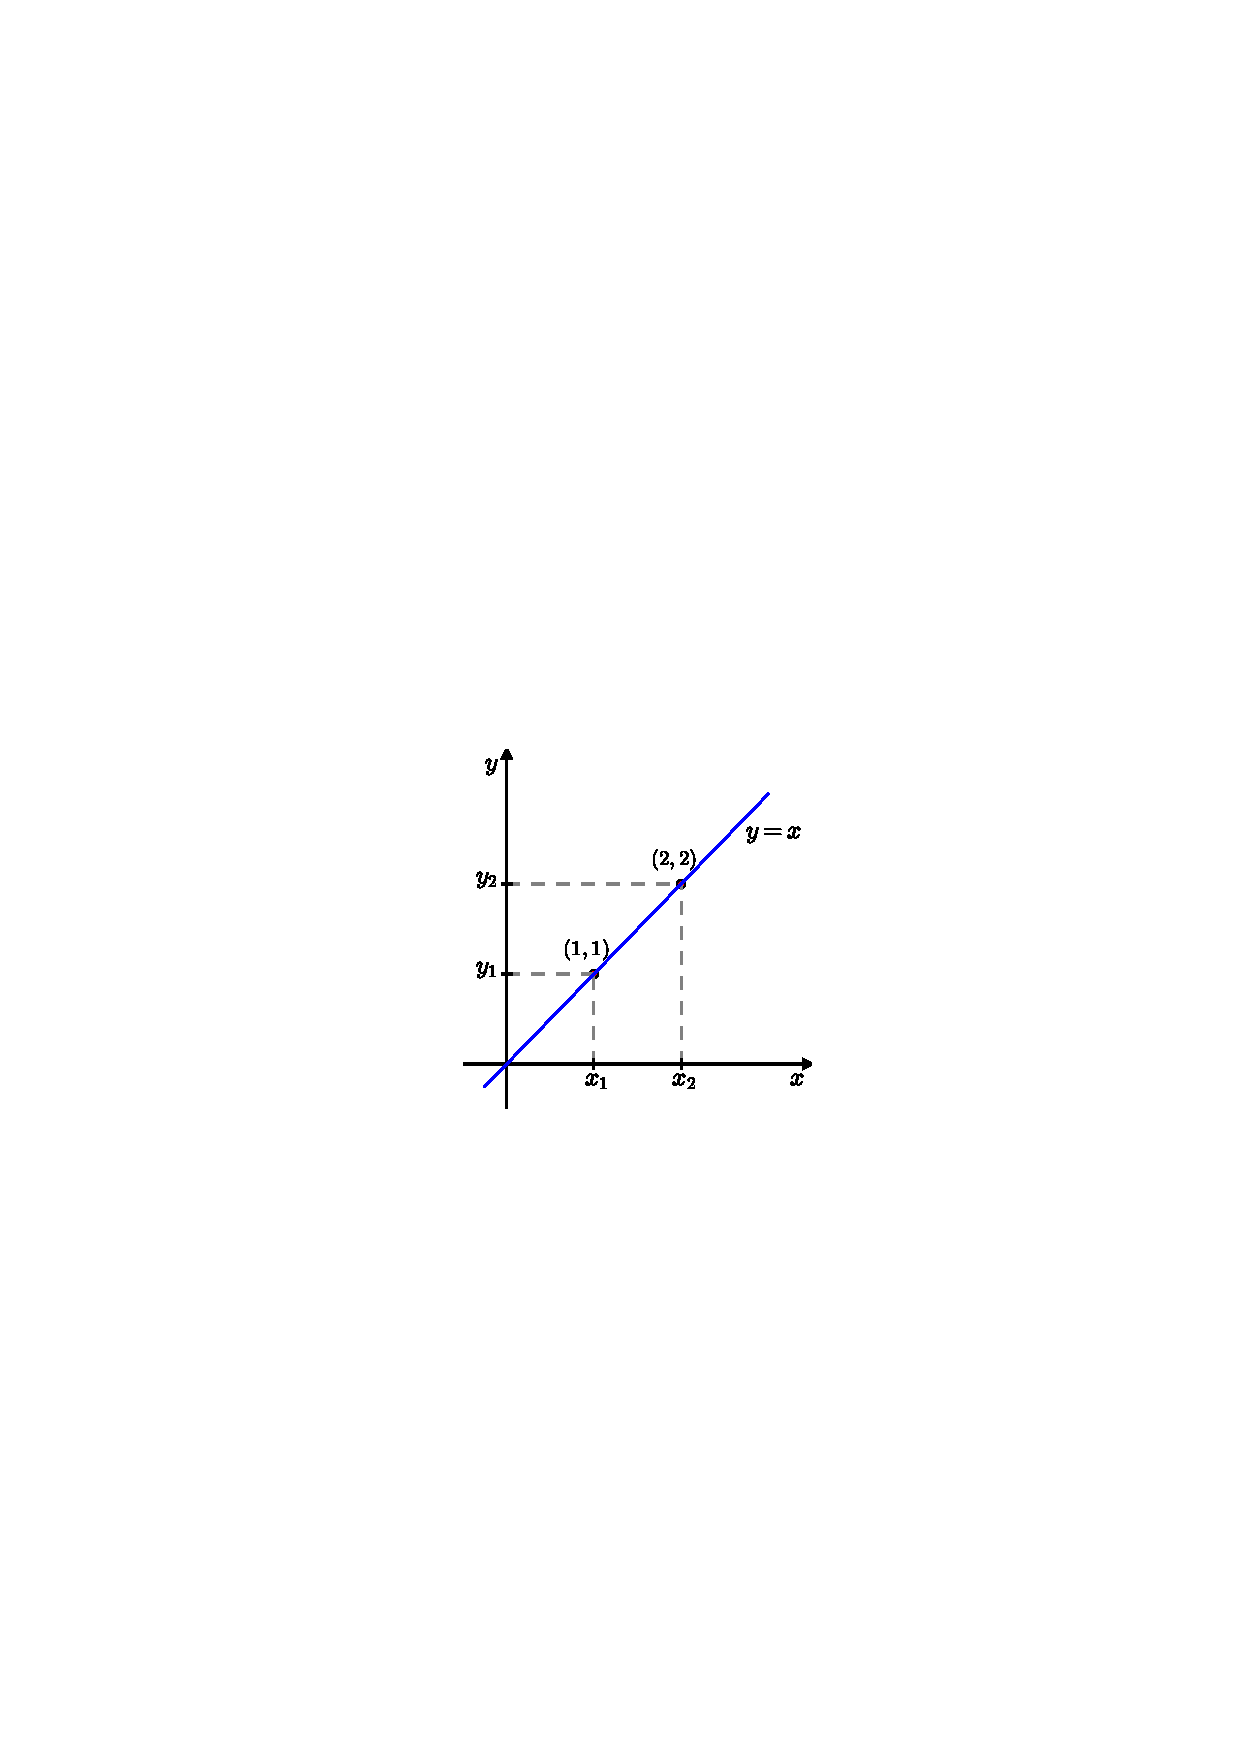
\includegraphics[scale=0.9]{./cap_interp/pics/ex_intro_interpolacao/ex_intro_interpolacao}
  \caption{Exemplo de interpolação de dois pontos por uma reta, veja o Exemplo~\ref{ex:intro_interpolacao}.}\label{fig:ex_intro_interp}
\end{figure}

\begin{ex}\label{ex:intro_interpolacao}
  Um dos problemas de interpolação mais simples é o de encontrar a equação da reta que passa por dois pontos dados. Por exemplo, sejam dados o conjunto de pontos $\{(1, 1), (2, 2)\}$ e a família de funções $\mathcal{F}_{[1,2]}$:
  \begin{equation}
   \mathcal{F}_{[1,2]} = \left\{f:[1,2]\rightarrow \mathbb{R}~;~[1,2]\ni x\mapsto f(x) = a + bx;\,a,b\in\mathbb{R}\right\}.
  \end{equation}
  Para que uma $f$ na família seja a função interpoladora do conjunto de pontos dados, precisamos que
  \begin{equation}
    \begin{array}{l}
      a + bx_1 = y_1\\
      a + bx_2 = y_2
    \end{array}\quad\text{isto é}\quad
    \begin{array}{l}
      a + b = 1\\
      a + 2b = 2
    \end{array}
  \end{equation}
o que nos fornece $a = 0$ e $b = 1$. Então, a função interpoladora $f$ é tal que  $f(x) = x$ para um $x\in[1,2]$. Os pontos e a reta interpolada estão esboçados na Figura~\ref{fig:ex_intro_interp}.
\end{ex}

Um problema de interpolação cuja a família de funções constitui-se de polinômios é chamado de problema de interpolação polinomial.

%%%%%%%%%%%%%%%%%%%%
% python
%%%%%%%%%%%%%%%%%%%%
\ifispython
Ao longo do capítulo, faremos alguns comentários usando códigos em \verb+Python 2.7+. Nestes, assumiremos que os seguintes módulos estão carregados:
\begin{verbatim}
from __future__ import division
import numpy as np
from numpy import linalg
from numpy.polynomial import polynomial as poly
\end{verbatim}
\fi
%%%%%%%%%%%%%%%%%%%%


\section{Interpolação polinomial}\index{interpolação!polinomial}

Interpolação polinomial é um caso particular do problema geral de interpolação, no qual a família de funções é constituída de polinômios. A escolha de polinômios como funções interpolantes é natural por diversos  motivos, entre eles: se $p$ é um polinômio de grau $n$, o valor $p(x)$ para um $x$ real é calculado através de $n+1$ operações de multiplicação e $n+1$ operações de adição. Para tanto, pode-se usar o algoritmo de Horner\footnote{William George Horner, 1786 - 1837, matemático britânico.}. Dado um polinômio $p$ de grau $n$ da forma
\begin{equation}
  p(x)=\sum_{k=0}^{n}a_k x^k,
\end{equation}
é possível reescrevê-lo como a sequência de operações dada por
\begin{equation}
  a_0 + x\left(a_1 + x\left(a_2 + x\left(\ldots + x\left(a_{n-1} + x a_n\right)\ldots\right)\right)\right).
\end{equation}

Também, derivadas e primitivas de polinômios são também polinômios cuja relação algébrica com o original é simples. Além disso, o teorema da aproximação de Weierstrass estabelece que qualquer função contínua definida em um intervalo fechado pode ser aproximada uniformemente por um polinômio tão bem quanto se queira.

\begin{teo}[Weierstrass]Seja $f$ uma função contínua definida no intervalo fechado $[a,b]$ e seja $\delta$ um número positivo. Então existe um polinômio $p$, tal que para todo $x\in[a,b]$,
  \begin{equation}
    |f(x)-p(x)|<\delta.
  \end{equation}
\end{teo}

Observe que para o problema ser bem determinado, é necessário restringirmos o grau dos polinômios. Dado um conjunto de $n$ pontos a serem interpolados $\{(x_i,y_i)\}_{i=1}^{n}$, $x_i\neq x_j$ para $i\neq j$, a família de polinômios $\mathcal{F} = \mathbb{P}_{n-1}$ deve ser escolhida, onde:
\begin{equation}
  \mathbb{P}_{n-1} := \left\{p : x\mapsto p(x) = \sum_{k=0}^{n-1}a_kx^k ;\, \{a_0,a_1,\ldots,a_{n-1}\}\in\mathbb{R}\right\},
\end{equation}
isto é, a família dos polinômios reais de grau menor ou igual a $n-1$.

O Exemplo~\ref{ex:intro_interpolacao} discute um dos casos mais simples de interpolação polinomial, o qual consiste em interpolar uma reta por dois pontos. Neste caso, a família de funções consiste de polinômios de grau 1. Se buscarmos interpolar uma parábola pelos dois pontos dados, o problema fica subdeterminado, pois existem infinitas parábolas que passam por dois pontos dados. Além disso, se buscarmos interpolar uma reta por três pontos dados, o problema estaria sobredeterminado e poderia não ter solução se os pontos não fossem colineares. Veja o Exercício~\ref{exer:problemas_mal_determinados}.

Assim, dado um conjunto com $n$ pontos $\{(x_i,y_i)\}_{i=1}^{n}$, chamamos de \emph{polinômio interpolador}\index{polinômio interpolador} o polinômio de grau menor ou igual a $n-1$ que os interpola.


\begin{figure}[ht]
  \centering
  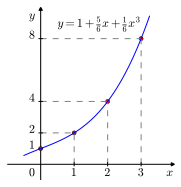
\includegraphics{./cap_interp/pics/ex_interpolacao_polinomial/ex_interpolacao_polinomial}
  \caption{Polinômio interpolador do conjunto de pontos $\{(0, 1)$, $(1, 6)$, $(2, 5)$, $(3, -8)\}$. Veja o Exemplo~\ref{ex:interpolacao_polinomial}.}\label{fig:ex_interpolacao_polinomial}
\end{figure}

\begin{ex}\label{ex:interpolacao_polinomial} Encontre o polinômio interpolador do conjunto de pontos $\{(0, 1)$, $(1, 6)$, $(2, 5)$, $(3, -8)\}$.
\end{ex}
\begin{sol}
Como o conjunto consiste de 4 pontos, o polinômio interpolador deve ser da forma:
\begin{equation}
  p(x) = a_0 + a_1x + a_2x^2 + a_3x^3.
\end{equation}
As condições de interpolação são $p(x_i) = y_i$, $i = 0, 1, 2, 3$, o que nos leva ao sistema linear:
\begin{equation}
  \begin{array}{lclclclcl}
    a_0& & & & & & &=&1\\
    a_0&+& a_1&+& a_2&+&  a_3&=&6\\
    a_0&+&2a_1&+&4a_2&+& 8a_3&=&5\\
    a_0&+&3a_1&+&9a_2&+&27a_3&=&-8
  \end{array}
\end{equation}
cuja solução é $a_0=1$, $a_1=6$, $a_2=0$ e $a_3=-1$. Portanto, o polinômio interpolador é $p(x)=1+6x-x^3$. Veja Figura~\ref{fig:ex_interpolacao_polinomial}.

%%%%%%%%%%%%%%%%%%%%
% scilab
%%%%%%%%%%%%%%%%%%%%
\ifisscilab
No \verb+Scilab+, podemos encontrar o polinômio interpolador e esboçar seu gráfico com os seguintes comandos:
\begin{verbatim}
-->xi = [0 1 2 3]';
-->yi = [1 6 5 -8]';
-->A = [xi.^0 xi.^1 xi.^2 xi.^3];
-->a = A\yi;
-->p = poly(a,'x','c')
  p  =
               3
     1 + 6x - x
-->xx = linspace(-0.5,3.25);
-->plot(xi,yi,'ro',xx,horner(p,xx),'b-');xgrid
\end{verbatim}
\fi
%%%%%%%%%%%%%%%%%%%%
%%%%%%%%%%%%%%%%%%%%
% octave
%%%%%%%%%%%%%%%%%%%%
\ifisoctave
No \verb+GNU Octave+, podemos encontrar o polinômio interpolador e esboçar seu gráfico com os seguintes comandos:
\begin{verbatim}
xi = [0 1 2 3]';
yi = [1 6 5 -8]';
A = [xi.^3 xi.^2 xi.^1 xi.^0];
a = A\yi;
xx = linspace(-0.5,3.25);
plot(xi,yi,'ro',xx,polyval(a,xx),'b-');xgrid
\end{verbatim}
\fi
%%%%%%%%%%%%%%%%%%%%
%%%%%%%%%%%%%%%%%%%%
% python
%%%%%%%%%%%%%%%%%%%%
\ifispython
Em \verb+Python+, podemos encontrar o polinômio interpolador e esboçar seu gráfico com os seguintes comandos:
\begin{verbatim}
>>> xi = np.array([0,1,2,3], dtype='double')
>>> yi = np.array([1,6,5,-8], dtype='double')
>>> A = np.array([xi**3,xi**2,xi**1,xi**0]).transpose()
>>> a = np.linalg.inv(A).dot(yi);a
array([ -1,  0.,  6,  1. ])
>>> xx = np.linspace(-0.5,3.25);
>>> plt.plot(xi,yi,'ro',xx,np.polyval(a,xx),'b-')
>>> plt.grid();plt.show()
\end{verbatim}
\fi
%%%%%%%%%%%%%%%%%%%%
\end{sol}


\begin{teo}\label{teo:interp_poli} Seja $\{(x_i,y_i)\}_{i=1}^{n}$ um conjunto de $n$ pares ordenados de números reais tais que $x_i \ne x_j$ se $i\ne j$, então existe um único polinômio $p(x)$ de grau $n-1$ ou inferior que passa por todos os pontos dados, isto é, $p(x_i)=y_i, i=1,\ldots, n$.
\end{teo}
\begin{proof} Observe que o problema de encontrar os coeficientes $a_0$, $a_1$,\ldots, $a_{n-1}$ do polinômio
\begin{equation} p(x)=a_0+a_1x+a_2x^2+\cdots a_{n-1}x^{n-1}=\sum_{k=0}^{n-1} a_k x^k \end{equation}
tal que $p(x_i)=y_i$ é equivalente a resolver o sistema linear com $n$ equações e $n$ incógnitas dado por
\begin{equation}
  \begin{split}
    a_0+a_1x_1+a_1x_1^2+\cdots +a_{n-1} x_1^{n-1} &= y_1,\\
    a_0+a_1x_2+a_2x_2^2+\cdots +a_{n-1} x_2^{n-1} &= y_2,\\
    &\vdots\\
    a_0+a_1x_n+a_2x_n^2+\cdots +a_{n-1} x_n^{n-1}&= y_n.
  \end{split}
\end{equation}
O qual pode ser escrito na forma matricial como
\begin{equation}
  \begin{bmatrix}
    1 & x_1 & x_1^2 & \cdots & x_1^{n-1}\\
    1 & x_2 & x_2^2 & \cdots & x_2^{n-1}\\
    1 & x_3 & x_3^2 & \cdots & x_3^{n-1}\\
    \vdots&\vdots&\vdots&\ddots&\vdots\\
    1 & x_n & x_n^2 & \cdots & x_n^{n-1}
  \end{bmatrix}
  \begin{bmatrix}
    a_0\\a_1\\a_2\\ \vdots \\a_{n-1}
  \end{bmatrix} =
  \begin{bmatrix}
    y_1\\y_2\\y_3\\ \vdots \\y_n
  \end{bmatrix}
\end{equation}
A matriz envolvida é uma \emph{matriz de Vandermonde}\footnote{Alexandre-Théophile Vandermonde, 1735 - 1796, matemático francês.}\index{matriz de Vandermonde} de ordem $n$ cujo determinante é dado pelo produtório duplo
\begin{equation} \prod_{1\leq i<j\leq n}\left(x_j-x_i\right) \end{equation}
É fácil ver que se as abscissas são diferentes dois a dois, então o determinante é não nulo. Disto decorre que a matriz envolvida é inversível e, portanto, o sistema possui uma solução que é única.
\end{proof}

% \begin{ex} Encontre o polinômio da forma $P(x)=a_0+a_1x+a_2x^2+a_3x^3$ que passa pelos pontos
% \begin{equation} (0,0),(1,1),(2,4),(3,9) \end{equation}
% Este problema é equivalente ao seguinte sistema linear:
% \begin{eqnarray*}
% a_0&=&0\\
% a_0+a_1+a_2+a_3&=&1\\
% a_0+2a_1+4a_2+8a_3&=&4\\
% a_0+3a_1+9a_2+27a_3&=&9
% \end{eqnarray*}
% cuja solução é $a_0=0$, $a_1=0$, $a_2=1$ e $a_3=0$. Portanto
% \begin{equation} P(x)=x^2 \end{equation}
% \end{ex}

Esta abordagem direta que usamos no Exemplo~\ref{ex:interpolacao_polinomial} e na demonstração do Teorema~\ref{teo:interp_poli} se mostra ineficiente quando o número de pontos é grande e quando existe grande variação nas abscissas. Neste caso, a matriz de Vandermonde é mal condicionada (ver \cite{Gautschi}), o que acarreta um aumento dos erros de arredondamento na solução do sistema.

Uma maneira de resolver este problema é escrever o polinômio em uma base que produza um sistema bem condicionado.

\subsection*{Exercícios resolvidos}

\construirExeresol

\begin{exeresol}\label{exeresol:problemas_mal_determinados}
  Mostre que:
  \begin{itemize}
  \item[a)] Existem infinitas parábolas que interpolam dois pontos dados $\{(x_1, y_1), (x_2, y_2)\}$, com $x_1 \neq x_2$.
  \item[b)] Não existe reta que interpola os pontos $\{(1, 1), (2, 2,1), (3, 3)\}$.
  \item[c)] Não existe parábola de equação $y = a_0 + a_1x + a_2x^2$ que interpola dois pontos dados $\{(x_1, y_1), (x_1, y_2)\}$, com $y_1 \neq y_2$. Mas, existem infinitas parábolas de equação $x = a_0 + a_1y + a_2y^2$ que interpolam estes pontos.
  \end{itemize}
\end{exeresol}
\begin{resol}
  \begin{itemize}
  \item[a)] Uma parábola de equação $y = a_1 + a_2x + a_3x^2$ que interpola os pontos deve satisfazer o sistema:
    \begin{equation}
      \begin{split}
        a_1 + a_2x_1 + a_3x_1^2 &= y_1\\
        a_1 + a_2x_2 + a_3x_2^2 &= y_2
      \end{split}
    \end{equation}
    Sem perda de generalidade, para cada $a_3\in\mathbb{R}$ dado, temos:
    \begin{equation}
      \begin{split}
        a_1 + a_2x_1  &= y_1 - a_3x_1^2\\
        a_1 + a_2x_2  &= y_2 - a_3x_2^2
      \end{split},
    \end{equation}
    o qual tem solução única, pois $x_1\neq x_2$. Ou seja, para cada $a_3\in\mathbb{R}$ dado, existem $a_1, a_2\in\mathbb{R}$ tais que a parábola de equação $y = a_1 + a_2x + a_3x^2$ interpola os pontos dados.
  \item[b)] Certamente não existem retas de equação $x = a$ que interpolam os pontos dados. Consideremos então retas de equação $y = a_1 + a_2x$. Para uma tal reta interpolar os pontos dados é necessário que:
    \begin{equation}
      \begin{split}
        a_1 + a_2 = 1\\
        a_1 + 2a_2 = 2,1\\
        a_1 + 3a_2 = 3
      \end{split},
    \end{equation}
    o qual é um sistema impossível.
  \item[c)] Não existe uma parábola de equação $y = a_1 + a_2x + a_3x^2$ que interpole os pontos dados, pois tal equação determina uma função de $x$ em $y$. Agora, para mostrar que existem infinitas parábolas de equação $x = a_1 + a_2y + a_3y^2$ que interpolam os pontos dados, basta seguir um raciocínio análogo ao do item a), trocando $x$ por $y$ e $y$ por $x$.
  \end{itemize}
\end{resol}

\subsection*{Exercícios}

\construirExer

\begin{exer}\label{exer:interp1}
Encontre o polinômio interpolador para o conjunto de pontos $\{(-2, -47)$, $(0, -3)$, $(1, 4)$, $(2, 41)\}$. Então, faça um gráfico com os pontos e o polinômio interpolador encontrado.
\end{exer}
\begin{resp}
  $p(x) = -3 + 2x + 5x^3$.
\end{resp}

\begin{exer}
  Encontre o polinômio interpolador para o conjunto de pontos $\{(-1, 1,25)$, $(0,5, 0,5)$, $(1, 1,25)$, $(1,25, 1,8125)\}$.
\end{exer}
\begin{resp}
  $p(x) = 0,25 + x^2$.
\end{resp}

\section{Diferenças divididas de Newton}\index{diferenças divididas de Newton}
Dado um conjunto com $n$ pontos $\{(x_i, y_i)\}_{i=1}^n$, o \emph{método das diferenças divididas de Newton} consiste em construir o polinômio interpolador da forma
\begin{equation}
  \begin{split}
    p(x) &= a_1 + a_2 (x-x_1) + a_3 (x-x_1)(x-x_2) + \cdots \\
         &+ a_n (x-x_1)(x-x_2)\cdots (x-x_{n-1}).
  \end{split}
\end{equation}
Como $p(x_i) = y_i$, $i=1, 2, \dotsc, n$, os coeficientes $a_i$ satisfazem o seguinte sistema triangular inferior:
\begin{small}
  \begin{equation}
    \begin{array}{ll}
a_1               &= y_1\\
a_1+a_2(x_2-x_1)  &= y_2\\
a_1+a_2(x_3-x_1)+a_3(x_3-x_1)(x_3-x_2) &= y_3\\
&\vdots\\
a_1+a_2(x_n-x_1)+\cdots + a_n(x_n-x_1)\cdots (x_n-x_{n-1}) &= y_n
    \end{array}
  \end{equation}
\end{small}
Resolvendo de cima para baixo, obtemos
\begin{equation}\label{eq:coef_dif_div}
  \begin{split}
a_1&=y_1\\
a_2&=\frac{y_2-a_1}{x_2-x_1}=\frac{y_2-y_1}{x_2-x_1}\\
a_3&=\frac{y_3-a_2(x_3-x_1)-a_1}{(x_3-x_1)(x_3-x_2)}=\frac{\frac{y_3-y_2}{(x_3-x_2)}-\frac{y_2-y_1}{(x_2-x_1)}}{(x_3-x_1)}\\
&\ldots
  \end{split}
\end{equation}

Note que os coeficientes são obtidos por diferenças das ordenadas divididas por diferenças das abscissas dos pontos dados. Para vermos isso mais claramente, introduzimos a seguinte notação:
\begin{eqnarray}
  f[x_j]&:=&y_j\\
  f[x_j, x_{j+1}]&:=&\frac{f[x_{j+1}]-f[x_j]}{x_{j+1}-x_j}\\
  f[x_j, x_{j+1}, x_{j+2}]&:=&\frac{f[x_{j+1}, x_{j+2}]-f[x_j, x_{j+1}]}{x_{j+2}-x_j}\\
        &\vdots&\\
  f[x_j, x_{j+1}, \dotsc, x_{j+k}] &:=& \frac{f[x_{j+1}, x_{j+2}, \dotsc, x_{j+k}]-f[x_j, x_{j+1}, \dotsc, x_{j+k-1}]}{x_{j+k}-x_j}
\end{eqnarray}
Chamamos $f[x_j]$ de diferença dividida de ordem zero (ou primeira diferença dividida), $f[x_i,x_j+1]$ de diferença dividida de ordem 1 (ou segunda diferença dividida) e assim por diante.

Uma inspeção cuidadosa dos coeficientes obtidos em \eqref{eq:coef_dif_div} nos mostra que
\begin{equation}
 a_k=f[x_1,x_2,\ldots,x_k]
\end{equation}
Isto nos permite esquematizar o método conforme apresentado na Tabela~\ref{tab:esquema_difdiv}.

\begin{table}
  \centering
  \caption{Esquema de diferenças divididas para um conjunto com três pontos $\{(x_i, y_i)\}_{i=1}^3$.}
  \label{tab:esquema_difdiv}
\begin{tabular}{c||c|ccc}\hline
$j$ & $x_j$ & $f[x_j]$ & $f[x_{j-1},x_j]$ & $f[x_{j-2},x_{j-1},x_j]$ \\\hline
$1$ & $x_1$ & $\pmb{f[x_1]}=y_1$ & &\\
&&&$\displaystyle \pmb{f[x_1,x_2]}=\frac{f[x_2]-f[x_1]}{x_2-x_1}$&\\
$2$ & $x_2$ & $f[x_2] = y_2$ && $\displaystyle \pmb{f[x_1,x_2,x_3]}=\frac{f[x_2,x_3]-f[x_1,x_2]}{x_3-x_1}$\\
&&&$\displaystyle f[x_2,x_3]=\frac{f[x_3]-f[x_2]}{x_3-x_2}$ &\\
$3$ & $x_3$ & $f[x_3]=y_3$ &&\\\hline
\end{tabular}
\end{table}

\begin{ex}
Use o método de diferenças divididas para encontrar o polinômio que passe pelos pontos $(-1,3),(0,1),(1,3),(3,43)$.
\end{ex}
\begin{sol}
Usando o esquema apresentado na Tabela~\ref{tab:esquema_difdiv}, obtemos
\begin{center}
\begin{tabular}{c||c|cccc}\hline
 $j$ & $x_j$ & $f[x_j]$ & $f[x_{j-1},x_j]$ & $f[x_{j-2},x_{j-1},x_j]$ & $f[x_{j-3},x_{j-2},x_{j-1},x_j]$\\\hline
$1$ & $-1$ & $\pmb{3}$&&&\\
&&&$\displaystyle \frac{1-3}{0-(-1)}=\pmb{-2}$&&\\
$2$&$0$&$1$&&$\displaystyle \frac{2-(-2)}{1-(-1)}=\pmb{2}$&\\
&&&$\displaystyle \frac{3-1}{1-0}=2$&&$\displaystyle\frac{6-2}{3-(-1)}=\pmb{1}$\\
$3$&$1$&$3$&&$\displaystyle \frac{20-2}{3-0}=6$&\\
&&&$\displaystyle \frac{43-3}{3-1}=20$&&\\
$4$&$3$&$43$&&&\\\hline
\end{tabular}
\end{center}
Portanto, o polinômio interpolador do conjunto de pontos dados é
\begin{equation}
  p(x) = 3-2(x+1)+2(x+1)x+(x+1)x(x-1)
\end{equation}
ou, equivalentemente, $p(x) = x^3+2x^2-x+1$.

%%%%%%%%%%%%%%%%%%%%
% octave
%%%%%%%%%%%%%%%%%%%%
\ifisoctave
No \verb+GNU Octave+, podemos fazer as contas acima da segunte forma:
\begin{verbatim}
x = [-1,0,1,3]';
y = [3,1,3,43]';
#inicializando a tabela
T = zeros(4,4);
#primeira coluna
T(:,1)=y;
#segunda coluna
T(2,2)=(T(2,1)-T(1,1))/(x(2)-x(1));
T(3,2)=(T(3,1)-T(2,1))/(x(3)-x(2));
T(4,2)=(T(4,1)-T(3,1))/(x(4)-x(3));
#terceira coluna
T(3,3)=(T(3,2)-T(2,2))/(x(3)-x(1));
T(4,3)=(T(4,2)-T(3,2))/(x(4)-x(2));
#quarta coluna
T(4,4)=(T(4,3)-T(3,3))/(x(4)-x(1));
#polinomio interpolador
p = T(1,1);
p = [0, p] + T(2,2)*[1,-x(1)];
p = [0, p] + T(3,3)*conv([1,-x(1)],[1,-x(2)]);
p = [0, p] + T(4,4)*conv(conv([1,-x(1)],[1,-x(2)]),[1,-x(3)]);
\end{verbatim}
\fi
%%%%%%%%%%%%%%%%%%%%
%%%%%%%%%%%%%%%%%%%%
% python
%%%%%%%%%%%%%%%%%%%%
\ifispython
Em \verb+Python+, podemos fazer as contas acima da segunte forma:
\begin{verbatim}
x = np.array([-1,0,1,3], dtype="double")
y = np.array([3,1,3,43], dtype="double")
#inicializando a tabela
T = np.zeros((4,4));
#primeira coluna
T[:,0]=y;
#segunda coluna
T[1,1]=(T[1,0]-T[0,0])/(x[1]-x[0]);
T[2,1]=(T[2,0]-T[1,0])/(x[2]-x[1]);
T[3,1]=(T[3,0]-T[2,0])/(x[3]-x[2]);
#terceira coluna
T[2,2]=(T[2,1]-T[1,1])/(x[2]-x[0]);
T[3,2]=(T[3,1]-T[2,1])/(x[3]-x[1]);
#quarta coluna
T[3,3]=(T[3,2]-T[2,2])/(x[3]-x[0]);
print(T)
#polinomio interpolador
p = np.array([T[0,0]], dtype="double")
paux = np.array([-x[0],1], dtype="double")
p.resize(2)
p += T[1,1]*paux
paux = poly.polymul(paux,[-x[1],1])
p.resize(3)
p += T[2,2]*paux
paux = poly.polymul(paux,[-x[2],1])
p.resize(4)
p += T[3,3]*paux
\end{verbatim}
\fi
%%%%%%%%%%%%%%%%%%%%
\end{sol}

\section{Polinômios de Lagrange}\index{polinômios!de Lagrange}
Outra maneira clássica de resolver o problema da interpolação polinomial é através dos polinômios de Lagrange. Dado um conjunto de pontos $\{x_j\}_{j=1}^n$ distintos dois a dois, definimos os polinômios de Lagrange como os polinômios de grau $n-1$ que satisfazem
\begin{equation}
L_k(x_j)=\left\{\begin{array}{rl}
1,& \text{se }k=j\\
0,& \text{se }k\neq j
\end{array}
\right.
\end{equation}
Assim, o polinômio $p(x)$ de grau $n-1$ que interpola os pontos dados, isto é, $p(x_j)=y_j, j=1,\ldots,n$ é dado por
\begin{equation}
  p(x)=y_1L_1(x)+y_2L_2(x)+\cdots +y_nL_n(x)=\sum_{k=1}^n y_k L_k(x).
\end{equation}

Para construir os polinômios de Lagrange, podemos analisar a sua forma fatorada, ou seja:
\begin{equation} L_k(x)=c_k\prod_{\substack{j=1\\j\ne i}}^{n} (x-x_j) \end{equation}
onde o coeficiente $c_k$ é obtido da condição $L_k(x_k)=1$:
\begin{equation} L_k(x_k)=c_k\prod_{\substack{j=1\\j\ne i}}^{n} (x_k-x_j) \Longrightarrow  c_k=\frac{1}{\displaystyle \prod_{\substack{j=1\\j\ne i}}^{n} (x_k-x_j)} \end{equation}
Portanto,
\begin{equation} L_k(x)=\prod_{\substack{j=1\\j\ne i}}^{n} \frac{(x-x_j)}{(x_k-x_j)} \end{equation}

\begin{obs} O problema de interpolação quando escrito usando como base os polinômios de Lagrange produz um sistema linear diagonal.
\end{obs}

\begin{ex}
  Encontre o polinômio da forma $p(x)=a_1+a_2x+a_3x^2+a_4x^3$ que passa pelos pontos $(0, 0)$, $(1, 1)$, $(2, 4)$, $(3, 9)$.
\end{ex}
\begin{sol}
Escrevemos:
\begin{eqnarray}
  L_1(x)&=& \frac{(x-1)(x-2)(x-3)}{(0-1)(0-2)(0-3)}=-\frac{1}{6}x^3+x^2-\frac{11}{6}x+1\\
  L_2(x)&=& \frac{x(x-2)(x-3)}{1(1-2)(1-3)}=\frac{1}{2}x^3-\frac{5}{2}x^2+3x\\
  L_3(x)&=& \frac{x(x-1)(x-3)}{2(2-1)(2-3)}=-\frac{1}{2}x^3+2x^2-\frac{3}{2}x\\
  L_4(x)&=& \frac{x(x-1)(x-2)}{3(3-1)(3-2)}=\frac{1}{6}x^3-\frac{1}{2}x^2+\frac{1}{3}x
\end{eqnarray}
Assim, temos:
\begin{equation}
  P(x)=0\cdot L_1(x)+1\cdot L_2(x)+4\cdot L_3(x)+9\cdot L_4(x)=x^2
\end{equation}

%%%%%%%%%%%%%%%%%%%%
% octave
%%%%%%%%%%%%%%%%%%%%
\ifisoctave
No \verb+GNU Octave+, podemos fazer as contas acima da segunte forma:
\begin{verbatim}
x = [0 1 2 3]';
y = [0 1 4 9]';
#L1
num = poly([x(2),x(3),x(4)]);
L1 = num/polyval(num,x(1));
#L2
num = poly([x(1),x(3),x(4)]);
L2 = num/polyval(num,x(2));
#L3
num = poly([x(1),x(2),x(4)]);
L3 = num/polyval(num,x(3));
#L4
num = poly([x(1),x(2),x(3)]);
L4 = num/polyval(num,x(4));
p = y(1)*L1 + y(2)*L2 + y(3)*L3 + y(4)*L4
\end{verbatim}
\fi
%%%%%%%%%%%%%%%%%%%%
\end{sol}

\section{Aproximação de funções reais por polinômios interpoladores}\index{aproximação!de funções!por polinômios}

\begin{teo}\label{teo_interp}
Dados $n+1$ pontos distintos, $x_0,\ x_1,\ \cdots,\ x_n$, dentro de um intervalo $[a,b]$ e uma função $f$ com $n+1$ derivadas contínuas nesse intervalo ($f\in C^{n+1}[a,b]$), então para cada $x$ em $[a,b]$, existe um número $\xi(x)$ em $(a,b)$ tal que
$$
f(x)=P(x)+\frac{f^{(n+1)}(\xi(x))}{(n+1)!}(x-x_0)(x-x_1)\cdots(x-x_n),
$$
onde $P(x)$ é o polinômio interpolador. Em especial, pode-se dizer que
$$
|f(x)-P(x)|\leq \frac{M}{(n+1)!}\left|(x-x_0)(x-x_1)\cdots(x-x_n)\right|,
$$
onde
$$
M=\max_{x\in[a,b]}|f^{(n+1)}(\xi(x))|
$$
\end{teo}

\begin{ex}
Considere a função $f(x)=\cos(x)$ e o polinômio $P(x)$ de grau 2 tal que $P(0)=\cos(0)=1$, $P(\frac{1}{2})=\cos(\frac{1}{2})$ e $P(1)=\cos(1)$. Use a fórmula de Lagrange para encontrar $P(x)$. Encontre o erro máximo que se assume ao aproximar o valor de $\cos(x)$ pelo de $P(x)$ no intervalo $[0,1]$. Trace os gráficos de $f(x)$ e $P(x)$ no intervalo $[0,1]$ no mesmo plano cartesiano e, depois, trace o gráfico da diferença $\cos(x)-P(x)$. Encontre o erro efetivo máximo $|\cos(x)-P(x)|$.
\end{ex}
\begin{sol}
  Usando polinômios de Lagrange, obtemos
  \begin{eqnarray}
    P(x) &=& 1\frac{(x-\frac{1}{2})(x-1)}{(0-\frac{1}{2})(0-1)}\nonumber\\
         &+& \cos\left(\frac{1}{2}\right)\frac{(x-0)(x-1)}{(\frac{1}{2}-0)(\frac{1}{2}-1)}\nonumber\\
         &+& \cos(1)\frac{(x-0)(x-\frac{1}{2})}{(1-0)(1-\frac{1}{2})}\\
         &\approx&   1 - 0,0299720583066x - 0,4297256358252x^2
  \end{eqnarray}

%%%%%%%%%%%%%%%%%%%%
% scilab
%%%%%%%%%%%%%%%%%%%%
\ifisscilab
No \verb+Scilab+, podemos computar o polinômio interpolador da seguinte forma:
\begin{verbatim}
L1=poly([.5 1],'x');L1=L1/horner(L1,0)
L2=poly([0 1],'x');L2=L2/horner(L2,0.5)
L3=poly([0 .5],'x');L3=L3/horner(L3,1)
P=L1+cos(.5)*L2+cos(1)*L3
x=[0:.05:1]
plot(x,cos)
plot(x,horner(P,x),'red')
plot(x,horner(P,x)-cos(x))
\end{verbatim}
\fi
%%%%%%%%%%%%%%%%%%%%
%%%%%%%%%%%%%%%%%%%%
% octave
%%%%%%%%%%%%%%%%%%%%
\ifisoctave
No \verb+GNU Octave+, podemos computar o polinômio interpolador da seguinte forma:
\begin{verbatim}
L1=poly([.5 1]);L1=L1/polyval(L1,0)
L2=poly([0 1]);L2=L2/polyval(L2,0.5)
L3=poly([0 .5]);L3=L3/polyval(L3,1)
P=L1+cos(.5)*L2+cos(1)*L3
\end{verbatim}
\fi
%%%%%%%%%%%%%%%%%%%%
%%%%%%%%%%%%%%%%%%%%
% python
%%%%%%%%%%%%%%%%%%%%
\ifispython
\construirPython
\fi
%%%%%%%%%%%%%%%%%%%%

Para estimar o erro máximo, precisamos estimar a derivada terceira de $f(x)$:
\begin{equation} |f'''(x)|=|\sin(x)|\leq \sin(1)<0,85 \end{equation}
e, assim,
$$
\max_{x\in[0,1]} \left|x\left(x-\frac{1}{2}\right)(x-1)\right|.
$$
O polinômio de grau três $Q(x)=x\left(x-\frac{1}{2}\right)(x-1)$ tem um mínimo (negativo) em $x_1=\frac{3+\sqrt{3}}{6}$ e um máximo (positivo) em $x_2=\frac{3-\sqrt{3}}{6}$. Logo:
$$
\max_{x\in[0,1]} \left|x\left(x-\frac{1}{2}\right)(x-1)\right|\leq \max\{|Q(x_1)|,\ |Q(x_2)|\}\approx 0,0481125.
$$
Portanto:
$$
|f(x)-P(x)|< \frac{0,85}{3!}0,0481125\approx 0,0068159<7\cdot 10^{-3}
$$

Para estimar o erro efetivo máximo, basta encontrar o máximo de $|P(x)-\cos(x)|$. O mínimo (negativo) de $P(x)-\cos(x)$ acontece em $x_1=4,29\cdot 10^{-3}$ e o máximo (positivo) acontece em $x_2=3,29\cdot 10^{-3}$. Portanto, o erro máximo efetivo é $4,29\cdot 10^{-3}$.
\end{sol}


\begin{ex}\label{exemp_simpson}
Considere o problema de aproximar o valor da integral $\int_0^1 f(x)dx$ pelo valor da integral do polinômio $P(x)$ que coincide com $f(x)$ nos pontos $x_0=0$, $x_1=\frac{1}{2}$ e $x_2=1$. Use a fórmula de Lagrange para encontrar $P(x)$. Obtenha o valor de $\int_0^1P(x)dx$ e encontre uma expressão para o erro de truncamento.
\end{ex}
O polinômio interpolador de $f(x)$ é
\begin{eqnarray*}
P(x)&=&f(0)\frac{(x-\frac{1}{2})(x-1)}{(0-\frac{1}{2})(0-1)}+f\left(\frac{1}{2}\right)\frac{(x-0)(x-1)}{(\frac{1}{2}-0)(\frac{1}{2}-1)}+f(1)\frac{(x-0)(x-\frac{1}{2})}{(1-0)(1-\frac{1}{2})}\\
&=&   f(0)(2x^2-3x+1)+f\left(\frac{1}{2}\right)(-4x^2+4x)+f(1)(2x^2-x)
\end{eqnarray*}
e a integral de $P(x)$ é:
\begin{eqnarray*}
\int_0^1 P(x)dx &=& \left[f(0)\left(\frac{2}{3}x^3 - \frac{3}{2}x^2+x\right)\right]_0^1 + \left[f\left(\frac{1}{2}\right)\left(-\frac{4}{3}x^3+2x^2\right)\right]_0^1 \\
&+& \left[f(1)\left(\frac{2}{3}x^3-\frac{1}{2}x^2\right)\right]_0^1\\
&=& f(0)\left(\frac{2}{3}-\frac{3}{2}+1\right)+f\left(\frac{1}{2}\right)\left(-\frac{4}{3}+2\right)+f(1)\left(\frac{2}{3}-\frac{1}{2}\right)\\
&=& \frac{1}{6}f(0)+\frac{2}{3}f\left(\frac{1}{2}\right)+\frac{1}{6}f(1)
\end{eqnarray*}
Para fazer a estimativa de erro usando o Teorema~\ref{teo_interp} e temos
\begin{eqnarray*}
\left|\int_0^1f(x)dx-\int_0^1 P(x)dx\right|&=&\left|\int_0^1f(x)- P(x)dx\right|\\
&\leq&\int_0^1|f(x)- P(x)|dx\\
&\leq& \frac{M}{6}  \int_0^1\left|x\left(x-\frac{1}{2}\right)(x-1)\right|dx\\
&=& \frac{M}{6}  \left[\int_0^{1/2}x\left(x-\frac{1}{2}\right)(x-1)dx\right.\\
&-&\left.\int_{1/2}^1x\left(x-\frac{1}{2}\right)(x-1)dx\right]\\
&=& \frac{M}{6}  \left[\frac{1}{64}-\left(-\frac{1}{64}\right)\right]=\frac{M}{192}.
\end{eqnarray*}
Lembramos que $M=\max_{x\in[0,1]}|f'''(x)|$.

\begin{obs}Existem estimativas melhores para o erro de truncamento para este esquema de integração numérica. Veremos com mais detalhes tais esquemas na teoria de integração numérica.
\end{obs}

\begin{ex}
Use o resultado do exemplo anterior para aproximar o valor das seguintes integrais:\\

a) $\displaystyle \int_0^1 \ln(x+1) dx$\\

b) $\displaystyle \int_0^1 e^{-x^2}dx$

\end{ex}
\begin{sol}
Usando a fórmula obtida, temos que
$$
\int_0^1\ln(x+1) dx \approx 0,39\pm \frac{1}{96}
$$
$$
\int_0^1 e^{-x^2} dx \approx 0,75\pm \frac{3,87}{192}
$$
\end{sol}

\subsection*{Exercícios}

\begin{exer}
  Use as mesmas técnicas usadas o resultado do Exemplo~\ref{exemp_simpson} para obter uma aproximação do valor de:
  \begin{equation}
    \int_0^1 f(x)dx
  \end{equation}
através do polinômio interpolador que coincide com $f(x)$ nos pontos $x=0$ e $x=1$.
\end{exer}
\begin{resp}

  $\int_0^1 P(x)dx =\frac{f(0)+f(1)}{2}$, $\frac{1}{12}\max_{x\in[0,1]}|f''(x)|$

\end{resp}

\section{Interpolação linear segmentada}\index{interpolação!linear segmentada}
Considere o conjunto $\left(x_i,y_i\right)_{j=1}^n$ de $n$ pontos. Assumiremos que $x_{i+1}>x_i$, ou seja, as abscissas são distintas e estão em ordem crescente. A função linear que interpola os pontos $x_i$ e $x_{i+1}$ no intervalo $i$ é dada por
\begin{equation} P_i(x)=y_i \frac{(x_{i+1}-x)}{(x_{i+1}-x_i)} + y_{i+1} \frac{(x-x_i)}{(x_{i+1}-x_i)} \end{equation}

O resultado da interpolação linear segmentada é a seguinte função contínua definida por partes no intervalo $[x_1,x_n]$:
\begin{equation} f(x)=P_i(x), ~~~~ x\in [x_i,x_{i+1}] \end{equation}

\begin{ex}
  Construa uma função linear por partes que interpola os pontos $(0,0)$, $(1,4)$, $(2,3)$, $(3,0)$, $(4,2)$, $(5,0)$.

A função procurada pode ser construída da seguinte forma:
\begin{equation}
  f(x) = \left\{
    \begin{array}{ll}
      0\frac{x-1}{0-1} + 1\frac{x-0}{1-0} ,& 0 \leq x < 1\\
      4\frac{x-2}{1-2} + 3\frac{x-1}{2-1} ,& 1 \leq x < 2\\
      3\frac{x-3}{2-3} + 0\frac{x-2}{3-2} ,& 2 \leq x < 3\\
      0\frac{x-4}{3-4} + 2\frac{x-3}{4-3} ,& 3 \leq x < 4\\
      2\frac{x-5}{4-5} + 0\frac{x-4}{5-4} ,& 4 \leq x \leq 5
    \end{array}
\right.
\end{equation}
Simplificando, obtemos:
\begin{equation}
  f(x) = \left\{
    \begin{array}{ll}
        x     ,& 0 \leq x < 1\\
       -x + 5 ,& 1 \leq x < 2\\
      -3x + 9 ,& 2 \leq x < 3\\
       2x - 6 ,& 3 \leq x < 4\\
      -2x +10 ,& 4 \leq x \leq 5
    \end{array}
\right.
\end{equation}
\end{ex}

A Figura~\ref{fig:linear_segmentada} é um esboço da função $f(x)$ obtida.

%%%%%%%%%%%%%%%%%%%%
% scilab
%%%%%%%%%%%%%%%%%%%%
\ifisscilab
Ela foi gerada no \verb+Scilab+ usando os comandos:
\verbatiminput{./cap_interp/codes/interpolacao_linear_segmentada/ex_linear_segmentada.sce}
\fi
%%%%%%%%%%%%%%%%%%%%

\begin{figure}[htp]
  \begin{center}
    \includegraphics[scale=0.5]{./cap_interp/pics/interpolacao_linear_segmentada.eps}
    \caption{Interpolação linear segmentada.}
    \label{fig:linear_segmentada}
  \end{center}
\end{figure}


\section{Interpolação cúbica segmentada - spline}\index{interpolação!cúbica segmentada}\index{spline}
A ideia empregada na interpolação linear segmentada pode ser estendida através da utilização de polinômios de grau superior. A escolha de polinômios de grau superior implica uma maior liberdade (há um número maior de coeficientes) na construção da interpolação. Parte dessa liberdade pode ser utilizada na exigência de suavidade para a interpolação.

\begin{defn}[spline de ordem $m$]Dado um conjunto de $n$ pontos $\mathcal{I}=\left\{(x_j,y_j)\right\}_{j=1}^n$ tais que $x_{j+1}>x_j$, ou seja, as abscissas são distintas e estão em ordem crescente; um spline de ordem $m$ que interpola estes pontos é uma função $s$ com as seguintes propriedades:
\begin{itemize}
\item[i)] Em cada intervalo $[x_j,x_{j+1})$, $j=1,2,\ldots n-2$ e no segmento $[x_{n-1},x_n]$ $s$ é um polinômio de grau menor ou igual a  $m$;
\item[ii)] Em algum dos intervalos $s$ é um polinômio de grau $m$;
\item[iii)] Em cada $x_j\in \mathcal{I}$, $s(x_j)=y_j$, isto é, o spline interpola os pontos dados;
\item[iv)] $s$ é uma função de classe $\mathcal{C}^{m-1}$, isto é, é função $m-1$ vezes continuamente diferenciável.
\end{itemize}
\end{defn}

São $n-1$ intervalos e em cada um deles há $m+1$ coeficientes a se determinar. As condições \textit{iii} e \textit{iv} impostas pela definição correspondem respectivamente a $n$ e $m(n-2)$ equações. Estas últimas, se devem à exigência de continuidade nos pontos internos, ou seja, os pontos de $\mathcal{I}$ com índices $j=2,3,\ldots,n-1$. Portanto, há $m-1$ coeficientes a mais do que o número de equações e, à exceção do caso $m=1$ (interpolação linear segmentada), o problema é subdeterminado. Ou seja, uma vez fixada a ordem $m>1$, existem infinitos splines de ordem $m$ que interpolam os pontos do conjunto $\mathcal{I}$.

O caso $m=3$, denominado spline cúbico, é de grande interesse pois reproduz o comportamento físico de réguas delgadas com estrutura elástica homogênea e perfil uniforme sujeitas aos vínculos representados pelos pontos  do conjunto $\mathcal{I}$. A equação diferencial que rege o comportamento do perfil dessas réguas é um caso particular do equação da viga de Euler-Bernoulli. Neste caso, a equação tem a forma
\begin{equation}\label{eq:ed-splin3}
\dfrac{d^4y}{dx^4}=0,
\end{equation}
cuja solução geral é um polinômio de grau 3.

Vamos supor que um spline cúbico que interpola o conjunto de pontos $\mathcal{I}$ é conhecido. Como esse spline é uma função de classe $\mathcal{C}^2$, as suas derivadas nos pontos do conjunto $\mathcal{I}$  são conhecidas também. Seja $y'_j$, o valor dessa derivada em $x=x_j$. Agora, vamos considerar dois pares de pontos sucessivos de $\mathcal{I}$,  $(x_j,y_j)$ e $(x_{j+1},y_{j+1})$. A forma do spline cúbico no intervalo $[x_j,x_{j+1})$ pode ser identificada com a solução da equação diferencial \eqref{eq:ed-splin3} no intervalo $(x_j,x_{j+1})$ sujeita às condições de contorno
\begin{equation}
y(x_j)=y_j,\quad y'(x_j)=y'_j,\quad y(x_{j+1})=y_{j+1}\quad\text{e}\quad y'(x_{j+1})=y'_{j+1}.
\end{equation}
A solução desse problema de contorno é escrita de modo conveniente como
\begin{equation}
s_j(x)=a_j+b_j(x-x_j)+c_j(x-x_j)^2+d_j(x-x_j)^3,
\end{equation}
onde as constantes $a_j$, $b_j$, $c_j$ e $d_j$ se relacionam às do problema de contorno.  As duas primeiras seguem imediatamente das condições de contorno em $x_j$:
\begin{equation}
a_j=y_j\quad\text{e}\quad b_j=y'_j.
\end{equation}
As duas últimas são obtidas pela solução do sistema de equações formado pelas condições de contorno em $x_{j+1}$:
\begin{equation}
c_j=3\frac{y_{j+1}-y_j}{\left(x_{j+1}-x_j\right)^2}-\frac{y'_{j+1}+2y'_j}{x_{j+1}-x_j} \quad\text{e}\quad d_j=-2\frac{y_{j+1}-y_j}{\left(x_{j+1}-x_j\right)^3}+\frac{y'_{j+1}+y'_j}{\left(x_{j+1}-x_j\right)^2}
\end{equation}
Esta relação entre o conjunto de valores para a derivada de um spline cúbico $\{y'_j\}_{j=1}^{n}$ nos pontos de interpolação $\mathcal{I}$ e os coeficientes dos polinômios em cada intervalo de interpolação pode ser resumida na seguinte proposição:
\begin{prop}
	Seja $s$ um spline cúbico que interpola o conjunto de pontos $\mathcal{I}=\{(x_j,y_j)\}_{j=1}^n\subset\mathbb{R}^2$ tais que $x_{j+1}>x_j$. Se $\{y'_j\}_{j=1}^n$ é o conjunto dos valores da derivada de $s$ em $x_j$, então em cada intervalo $[x_j,x_{j+1})$ (fechado também à direita quando $j=n-1$) o spline é igual a $s_j$:
	\begin{equation}\label{eq:spline3}
	s_j(x)=a_j+b_j(x-x_j)+c_j(x-x_j)^2+d_j(x-x_j)^3,
	\end{equation}
	onde
	\begin{equation}
	\begin{array}{ll}\label{eq:spline3-coef}
		a_j=y_j,&c_j=3\dfrac{y_{j+1}-y_j}{h_j^2}-\dfrac{y'_{j+1}+2y'_j}{h_j},\\
		b_j=y'_j,&d_j=-2\dfrac{y_{j+1}-y_j}{h_j^3}+\dfrac{y'_{j+1}+y'_j}{h_j^2}
	\end{array}
	\end{equation}
	e
	\begin{equation}\label{eq:espacamento}
		h_j=x_{j+1}-x_j,\quad j=1,2,\ldots,n-1
	\end{equation}
	é a distância entre as abscissas de dois pontos de interpolação consecutivos.
\end{prop}
De acordo com a proposição anterior, toda informação sobre um spline cúbico é armazenada no conjunto $\{(x_j,y_j,y'_j)\}_{j=1}^n$. Por construção, uma função $s$ definida a partir de \eqref{eq:spline3}, \eqref{eq:spline3-coef} e \eqref{eq:espacamento} com um conjunto $\{(x_j,y_j,y'_j)\}_{j=1}^n\subset\mathbb{R}^3$, onde $x_{j+1}>x_j$ é de classe $\mathcal{C}^1$ mas não necessariamente um spline cúbico. Para ser um spline cúbico, os valores do conjunto $\{y'_j\}_{j=1}^n$ devem garantir a continuidade da derivada segunda de $s$ em todo intervalo $(x_1,x_n)$. Ou seja, devemos ter
\begin{equation}
\lim\limits_{x\nearrow x_{j+1} }s''_j(x)=s''_{j+1}(x_{j+1})
\end{equation}
em todos os pontos internos $j=1,2,\ldots,n-2$.  Em termos dos coeficientes dos polinômios cúbicos \eqref{eq:spline3}, a equação anterior assume a forma
\begin{equation}
2c_j+6d_jh_j=2c_{j+1},\quad j=1,2,\ldots,n-2.
\end{equation}
Esta última equação e \eqref{eq:spline3-coef} permitem construir um sistema de equações lineares para as variáveis $y'_j$:
\begin{prop} Dado o conjunto de pontos $\mathcal{I}=\{(x_j,y_j)\}_{j=1}^n\subset\mathbb{R}^2$ tais que $x_{j+1}>x_j$, as derivadas de um spline cúbico que interpola os pontos $\mathcal{I}$, $y'_j$, $j=1,2,\ldots,n$ satisfazem o sistema de equações algébricas lineares
\begin{equation}\label{eq:spline3-der}
h_jy'_{j-1}+2(h_{j-1}+h_j)y'_j+h_{j-1}y'_{j+1}=3\left(h_j\dfrac{y_j-y_{j-1}}{h_{j-1}}+h_{j-1}\dfrac{y_{j+1}-y_j}{h_j}\right),
\end{equation}
onde $j=2,3,\ldots,n-1$ e $h_j=x_{j+1}-x_j$.
\end{prop}
O sistema de equações \eqref{eq:spline3-der} é subdeterminado. São $n$ variáveis e $n-2$ equações. A inclusão de duas equações adicionais linearmente independentes das $n-2$ equações \eqref{eq:spline3-der} possibilita a existência de uma única solução. Tipicamente essas equações adicionais envolvem o comportamento do spline na fronteira ou na sua vizinhança.  A seguir, veremos quatro escolhas mais conhecidas.


\subsection{Spline natural}\index{spline!natural}

Uma forma de definir as duas equações adicionais para completar o sistema \eqref{eq:spline3-der} é impor condições de fronteira livres (ou naturais), ou seja,
\begin{equation}
s''(x_1)=s''(x_n)=0.
\end{equation}
De acordo com \eqref{eq:spline3} essas equações implicam respectivamente
\begin{equation}
c_1=0\quad\text{e}\quad 2c_{n-1}+6d_{n-1}h_{n-1}=0,
\end{equation}
ou seja,
\begin{equation}
	\left\{\begin{array}{l}
		2y'_1+y'_2=3\dfrac{y_2-y_1}{h_1}\\
		\\
		y'_{n-1}+2y'_n=3\dfrac{y_n-y_{n-1}}{h_{n-1}}
	\end{array}\right..
\end{equation}
Essas duas equações em conjunto com as equações \eqref{eq:spline3-der} formam um sistema de $n$ equações algébricas lineares $Ay'=z$, onde
\begin{equation}
	\begin{scriptsize}
		A=\left[\begin{array}{ccccccc}
			2 &1&0&0 &\cdots&0&0\\
			h_2&2(h_1+h_2)&h_1&0&\cdots&0&0\\
			0&h_3&2(h_2+h_3)&h_2&\cdots&0&0\\
			\vdots&\vdots&\vdots&\vdots&\ddots&\vdots&\vdots\\
			0&0&0&\cdots&h_{n-1} & 2(h_{n-1}+h_{n-2})&h_{n-2}\\
			0&0&0&\cdots &0&1&2
		\end{array}\right] ,
	\end{scriptsize}
\end{equation}
\begin{equation}
	y' = \left[\begin{array}{c}
		y'_1\\
		y'_2\\
		\vdots\\
		y'_n
	\end{array}\right]\qquad \text{e}\qquad
	z = 3\left[\begin{array}{c}
		\frac{y_2-y_1}{h_1}\\
		h_2\frac{y_2-y_1}{h_1}+h_1\frac{y_3-y_2}{h_2}\\
		h_3\frac{y_3-y_2}{h_2}+h_2\frac{y_4-y_3}{h_3}\\
		\vdots\\
		h_{n-1}\frac{y_{n-1}-y_{n-2}}{h_{n-2}}+h_{n-2}\frac{y_n-y_{n-1}}{h_{n-1}}\\
		\frac{y_n-y_{n-1}}{h_{n-1}}
	\end{array}\right].
\end{equation}
Observe que a matriz $A$ é diagonal dominante estrita e, portanto, o sistema $Ay'=z$ possui solução única. Calculado $y'$, os valores dos $a_j$, $b_j$, $c_j$ e $d_j$ são obtidos diretamente pelas expressões \eqref{eq:spline3-coef}.

\begin{ex}Construa um spline cúbico natural que passe pelos pontos $(2,~4,5)$, $(5,-1,9)$, $(9,~0,5)$ e $(12,-0,5)$.
\end{ex}
\begin{sol}
O spline desejado é uma função definida por partes da forma:
\begin{equation}
	s(x)=\left\{\begin{array}{ll}
		a_1+b_1(x-2)+c_1(x-2)^2+d_1(x-2)^3 ,& 2\leq x <5\\
	    a_2+b_2(x-5)+c_2(x-5)^2+d_2(x-5)^3 ,& 5\leq x <9\\
	    a_3+b_3(x-9)+c_3(x-9)^2+d_3(x-9)^3 ,& 9\leq x \leq 12
	\end{array}\right..
\end{equation}
As variáveis $y'_1$, $y'_2$, $y'_3$ e $y'_4$ resolvem o sistema $Ay' = z$, onde
\begin{equation}
	A = \begin{bmatrix}
		2 &1&0&0 \\
		4&2(4+3)&3&0\\
		0&3&2(3+4)&4\\
		0&0&1&2
	\end{bmatrix} = \begin{bmatrix}
		2 &1&0&0 \\
		4&14&3&0\\
		0&3&14&4\\
		0&0&1&2
	\end{bmatrix}  ,
\end{equation}
\begin{equation}
	y = \begin{bmatrix}
		y'_1\\
		y'_2\\
		y'_3\\
		y'_4
	\end{bmatrix} \quad \text{e}\quad
	z = 3\begin{bmatrix}
		\frac{1}{3}(-1,9-4,5)\\
		\frac{4}{3}(-1,9-4,5)+\frac{3}{4}(0,5-(-1,9))\\
		\frac{3}{4}(0,5-(-1,9))+\frac{4}{3}(-0.5-(0,5))\\
		\frac{1}{3}(-0,5-(0.5))
	\end{bmatrix} = \begin{bmatrix}
		-6,4\\
		-20,2\\
		1,4\\
		-1
	\end{bmatrix} .
\end{equation}
A solução é  $y'_1=-2,8\bar{3}$, $y'_2=-0,7\bar{3}$, $y'_3=0,4\bar{6}$ e $y'_4=-0,7\bar{3}$. Calculamos os coeficientes usando as expressões \eqref{eq:spline3-coef}:
\begin{equation}
	\begin{array}{lclclcl}
		a_1&=&y_1=4,5,& \qquad&b_1 &=&y'_1=-2,8\bar{3}, \\
		a_2&=&y_2=-1,9,& \qquad&b_2&=&y'_2=-0,7\bar{3}, \\
		a_3&=&y_3=0,5.& \qquad&b_3&=&y'_3=0,4\bar{6}, \\
		&&&&&&\\
		c_1&=&0,& \qquad&d_1&=&0,0\bar{7}, \\
		c_2&=&0,7,& \qquad&d_2&=&-0,091\bar{6}, \\
		c_3&=&-0,4,& \qquad&d_3&=&0,0\bar{4}.
	\end{array}
\end{equation}
Portanto:
\begin{small}
	\begin{equation}
		S(x)=\left\{\begin{array}{ll}
			4,5-2,8\bar{3}(x-2)+0,0\bar{7}(x-2)^3 &\!, 2\leq x<5\\
			-1,9-0,7\bar{3}(x-5)+0,7(x-5)^2-0,091\bar{6}(x-5)^3 &\!, 5\leq x<9\\
			0,5+0,4\bar{6}(x-9)-0,4(x-9)^2+0,0\bar{4}(x-9)^3 &\!, 9\leq x\leq 12
		\end{array}\right. .
	\end{equation}
\end{small}

%%%%%%%%%%%%%%%%%%%%
% scilab
%%%%%%%%%%%%%%%%%%%%
\ifisscilab
No \verb+Scilab+, podemos utilizar:
\begin{verbatim}
xi = [2;5;9;12]
yi = [4.5;-1.9;0.5;-0.5]
hi = xi(2:4)-xi(1:3)
A = [2 1 0 0;hi(2) 2*(hi(1)+hi(2)) hi(1) 0; ...
   0 hi(3) 2*(hi(2)+hi(3)) hi(2);0 0 1 2 ]
z = 3*[(yi(2)-yi(1))/hi(1); ...
   hi(2)/hi(1)*(yi(2)-yi(1))+hi(1)/hi(2)*(yi(3)-yi(2));...
   hi(3)/hi(2)*(yi(3)-yi(2))+hi(2)/hi(3)*(yi(4)-yi(3));...
   (yi(4)-yi(3))/hi(3)]
dyi = A\z
a=yi(1:3)
b=dyi(1:3)
c(1)=0
c(2:3)=3*(yi(3:4)-yi(2:3))./hi(2:3).^2 ...
         - (dyi(3:4)+2*dyi(2:3))./hi(2:3)
d=-2*(yi(2:4)-yi(1:3))./hi.^3 + (dyi(2:4)+dyi(1:3))./hi.^2
for i=1:3
    P(i) = poly([a(i) b(i) c(i) d(i)],'x','coeff')
    z = [xi(i):.01:xi(i+1)]
    plot(z,horner(P(i),z-xi(i)))
end
\end{verbatim}

O mesmo resultado é obtido através das instruções \verb+splin+ e \verb+interp+ do \verb+Scilab+:
\begin{verbatim}
xi = [2;5;9;12]
yi = [4.5;-1.9;0.5;-0.5]
dyi=splin(xi,yi,'natural')
z=linspace(xi(1),xi($))
plot(z,interp(z,xi,yi,dyi))
\end{verbatim}
\fi
%%%%%%%%%%%%%%%%%%%%
\end{sol}

\subsection{Spline fixado}\index{spline!fixado}

O spline fixado $s$ é obtido pela escolha dos valores das derivadas nas extremidades do intervalo de interpolação. Isto diminui o número de variáveis para $n-2$ pois $y'_1$ e $y'_n$ deixam de ser incógnitas.

As equações \eqref{eq:spline3-der} formam um sistema de $n-2$ equações $Ay' = z$, onde
\begin{equation}
	\begin{scriptsize}
		A=\left[\begin{array}{ccccccc}
			2(h_1+h_2)&h_1&0&0 &\cdots&0&0\\
			h_3&2(h_2+h_3)&h_2&0&\cdots&0&0\\
			0&h_4&2(h_3+h_4)&h_3&\cdots&0&0\\
			\vdots&\vdots&\vdots&\vdots&\ddots&\vdots&\vdots\\
			0&0&0&\cdots&h_{n-2} & 2(h_{n-3}+h_{n-2})&h_{n-3}\\
			0&0&0&\cdots &0&h_{n-1}&2(h_{n-2}+h_{n-1})
		\end{array}\right],
	\end{scriptsize}
\end{equation}
\begin{equation}
	\begin{small}
		y'= \left[\begin{array}{c}
			y'_2\\
			y'_3\\
			\vdots\\
			y'_{n-1}
		\end{array}\right]\qquad \text{e}\qquad
		z = 3\left[\begin{array}{c}
			h_2\frac{y_2-y_1}{h_1}+h_1\frac{y_3-y_2}{h_2}-h_2y'_1\\
			h_3\frac{y_3-y_2}{h_2}+h_2\frac{y_4-y_3}{h_3}\\
			\vdots\\
			h_{n-2}\frac{y_{n-2}-y_{n-3}}{h_{n-3}}+h_{n-3}\frac{y_{n-1}-y_{n-2}}{h_{n-2}}\\
			h_{n-1}\frac{y_{n-1}-y_{n-2}}{h_{n-2}}+h_{n-2}\frac{y_n-y_{n-1}}{h_{n-1}}-h_{n-2}y'_n
		\end{array}\right].
	\end{small}
\end{equation}
Observe que a matriz $A$ é diagonal dominante estrita e, portanto, o sistema $Ay' = z$ possui solução única.

%\begin{ex}Construa um spline cúbico com fronteira fixada que interpola a função $y=\sin (x)$ nos pontos $x=0$, $x=\frac{\pi}{2}$, $x=\pi$, $x=\frac{3\pi}{2}$ e $x=2\pi$.
%\end{ex}
%O spline desejado passa pelos pontos $(0,0)$, $(\pi/2,1)$, $(\pi,0)$, $(3\pi/2,-1)$ e $(2\pi,0)$ e tem a forma:
%\begin{equation}
%S(x)=\left\{\begin{array}{ll}
%a_1+b_1x+c_1x^2+d_1x^3,& 0\leq x<\frac{\pi}{2}\\
%a_2+b_2(x-\frac{\pi}{2})+c_2(x-\frac{\pi}{2})^2+d_2(x-\frac{\pi}{2})^3,& \frac{\pi}{2}\leq x<\pi\\
%a_3+b_3(x-\pi)+c_3(x-\pi)^2+d_3(x-\pi)^3,& \pi\leq x<\frac{3\pi}{2}\\
%a_4+b_4(x-\frac{3\pi}{2})+c_4(x-\frac{3\pi}{2})^2+d_4(x-\frac{3\pi}{2})^3,& \frac{3\pi}{2}\leq x\leq 2\pi
%\end{array}\right..
%\end{equation}
%Observe que ele satisfaz as condição de contorno $f'(0)=\cos(0)=1$ e $f'(2\pi)=\cos(2\pi)=1$.

%Os coeficientes $c_1$, $c_2$, $c_3$ e $c_4$ resolvem o sistema $Ac = z$, onde:
%\begin{equation}
%A=\left[\begin{array}{ccccc}
%\pi &\pi/2&0&0&0 \\
%\pi/2&2\pi&\pi/2&0&0\\
%0&\pi/2&2\pi&\pi/2&0\\
%0&0&\pi/2&2\pi&\pi/2\\
%0&0&0&\pi/2&\pi\\
%\end{array}\right]
%\end{equation}
%\begin{equation}
%c = \left[\begin{array}{c}
%c_1\\
%c_2\\
%c_3\\
%c_4\\
%c_5
%\end{array}\right]\qquad \text{e}\qquad
%z = \left[\begin{array}{c}
%3\frac{1-0}{\pi/2}-3\cdot 1\\
%3\frac{0-1}{\pi/2}-3\frac{1-0}{\pi/2}\\
%3\frac{-1-0}{\pi/2}-3\frac{0-1}{\pi/2}\\
%3\frac{0-(-1)}{\pi/2}-3\frac{(-1)-0}{\pi/2}\\
%3\cdot 1-3\frac{0-(-1)}{\pi/2}
%\end{array}\right]=\left[\begin{array}{c}
%6/\pi-3\\
%-12/\pi\\
%0\\
%12/\pi\\
%3-6/\pi
%\end{array}\right]
%\end{equation}
%Aqui $c_5$ é um coeficiente artificial para o problema. A solução é  $c_1=-0,0491874$, $c_2=-0,5956302$, $c_3=0$, $c_4=0,5956302$ e $c_5=0,0491874$. Calculamos os demais coeficientes usando as expressões \eqref{eq_an_spline}, \eqref{eq_bn_spline} e \eqref{eq_dn_spline}:
%\begin{eqnarray*}
%a_1&=&y_1=0\\
%a_2&=&y_2=1\\
%a_3&=&y_3=0\\
%a_4&=&y_3=-1\\
%\end{eqnarray*}
%\begin{eqnarray*}
%d_1&=&\frac{c_{2}-c_1}{3h_1}=\frac{-0,5956302-(-0,0491874)}{3\cdot \pi/2}=-0,1159588\\
%d_2&=&\frac{c_{3}-c_2}{3h_2}=\frac{0-(-0,5956302)}{3\cdot \pi/2}=0,1263967\\
%d_3&=&\frac{c_{4}-c_3}{3h_3}=\frac{0,5956302- 0}{3\cdot \pi/2}=0,1263967\\
%d_4&=&\frac{c_{5}-c_4}{3h_4}=\frac{0,0491874- 0,5956302}{3\cdot \pi/2}=-0,1159588
%\end{eqnarray*}
%\begin{eqnarray*}
%b_1&=& \frac{y_{2}-y_1}{h_1}-\frac{h_1}{3}(2c_1+c_{2})\\
%&=&\frac{1-0}{\pi/2}-\frac{\pi/2}{3}(2\cdot (-0,0491874)-0,5956302)=1\\
%b_2&=&\frac{y_{3}-y_2}{h_2}-\frac{h_2}{3}(2c_2+c_{3})\\
%&=&\frac{0-1}{\pi/2}-\frac{\pi/2}{3}(2\cdot(-0,5956302) +0)=-0,0128772\\
%b_3&=&\frac{y_{4}-y_3}{h_3}-\frac{h_3}{3}(2c_3+c_{4})\\
%&=&\frac{-1-0}{\pi/2}-\frac{\pi/2}{3}(2\cdot 0+0,5956302)=-0,9484910\\
%b_4&=&\frac{y_{5}-y_4}{h_4}-\frac{h_4}{3}(2c_4+c_{5})\\
%&=&\frac{0-(-1)}{\pi/2}-\frac{\pi/2}{3}(2\cdot 0,5956302+0,0491874)=-0,0128772
%\end{eqnarray*}
%Portanto,
%\begin{small}
%\begin{equation}
%S(x)=\left\{\begin{array}{ll}
%x-0,049x^2-0,12x^3,& 0\leq x<\frac{\pi}{2}\\
%1+-0,01(x-\frac{\pi}{2})-0,6(x-\frac{\pi}{2})^2+0,13(x-\frac{\pi}{2})^3,& \frac{\pi}{2}\leq x<\pi\\
%-0,95(x-\pi)+0,13(x-\pi)^3,& \pi\leq x<\frac{3\pi}{2}\\
%-1-0,01(x-\frac{3\pi}{2})+0,6(x-\frac{3\pi}{2})^2-0,12(x-\frac{3\pi}{2})^3,& \frac{3\pi}{2}\leq x\leq2\pi
%\end{array}\right.
%\end{equation}
%\end{small}

%\ifisscilab
%No \verb+Scilab+, podemos resolver este problema fazendo:
%\verbatiminput{./cap_interp/codes/splines/ex_spline_fixado.sce}
%\fi

\subsection{Spline \textit{not-a-knot}}\index{spline!not-a-knot}

O spline \textit{not-a-knot} é definido com um spline cúbico que satisfaz as equações adicionais
\begin{equation}
	\lim\limits_{x\nearrow x_2 }s'''_1(x)=s'''_2(x_2)\quad\text{e}\quad	\lim\limits_{x\nearrow x_{n-1} }s'''_{n-2}(x)=s'''_{n-1}(x_{n-1}).
\end{equation}
Em termos dos coeficientes \eqref{eq:spline3}, as equações anteriores correspondem a
\begin{equation}
	d_1=d_2\quad\text{e}\quad d_{n-2}=d_{n-1},
\end{equation}
ou seja,
\begin{equation}
\left\{\begin{array}{l}
	h_2^2y'_1+(h_2^2-h_1^2)y'_2-h_1^2y'_3=2\left(h_2^2\dfrac{y_2-y_1}{h_1}-h_1^2\dfrac{y_3-y_2}{h_2}\right)\\
	\\
	h_{n-1}^2y'_{n-2}+(h_{n-1}^2-h_{n-2}^2)y'_{n-1}-h_{n-2}^2y'_n=2\left(h_{n-1}^2\dfrac{y_{n-1}-y_{n-2}}{h_{n-2}}-h_{n-2}^2\dfrac{y_n-y_{n-1}}{h_{n-1}}\right)
	\end{array}\right..
\end{equation}
Essas duas equações agregadas às equações \eqref{eq:spline3-der} formam um sistema de $n$ equações $Ay' = z$, onde
\begin{equation}
	\begin{scriptsize}
		A=\left[\begin{array}{ccccccc}
			h_2^2&h_2^2-h_1^2&-h_1^2&0&\cdots&0&0\\
			h_2&2(h_1+h_2)&h_1&0&\cdots&0&0\\
			0&h_3&2(h_2+h_3)&h_2&\cdots&0&0\\
			\vdots&\vdots&\vdots&\vdots&\ddots&\vdots&\vdots\\
			0&0&0&\cdots&h_{n-1} & 2(h_{n-2}+h_{n-1})&h_{n-2}\\
			0&0&0&\cdots &h_{n-1}^2&h_{n-1}^2-h_{n-2}^2&-h_{n-2}^2
		\end{array}\right],
	\end{scriptsize}
\end{equation}
\begin{equation}
	\begin{small}
		y'= \left[\begin{array}{c}
			y'_1\\
			y'_2\\
			\vdots\\
			y'_n
		\end{array}\right]\qquad \text{e}\qquad
		z = \left[\begin{array}{c}
			2\left(h_2^2\dfrac{y_2-y_1}{h_1}-h_1^2\dfrac{y_3-y_2}{h_2}\right)\\
			3\left(h_2\frac{y_2-y_1}{h_1}+h_1\frac{y_3-y_2}{h_2}\right)\\
			\vdots\\
			3\left(h_{n-1}\frac{y_{n-1}-y_{n-2}}{h_{n-2}}+h_{n-2}\frac{y_n-y_{n-1}}{h_{n-1}}\right)\\
			2\left(h_{n-1}^2\dfrac{y_{n-1}-y_{n-2}}{h_{n-2}}-h_{n-2}^2\dfrac{y_n-y_{n-1}}{h_{n-1}}\right)\\
		\end{array}\right].
	\end{small}
\end{equation}
Se reduzirmos esse sistema pela eliminação das incógnitas $y'_1$ e $y'_n$, o sistema resultante possui uma matriz de coeficientes diagonal dominante estrita, portanto, a solução é única.

O termo \textit{not-a-knot} (não nó) relaciona-se à nomenclatura dos splines. O termo \textit{nó} é utilizado para os pontos interpolados. Neles, a derivada terceira da função spline é descontínua, portanto, quando impomos a continuidade dessa derivada em $x_2$ e $x_{n-1}$ é como se esses pontos deixassem de ser nós.

\subsection{Spline periódico}\index{spline!periódico}
Se o conjunto de $n$ pontos da interpolação $\mathcal{I}$ for tal que $y_1=y_n$, então é possível construir o spline periódico, definido com um spline cúbico que satisfaz as seguintes condições de periodicidade
\begin{equation}
	s'_1(x_1)=s'_{n-1}(x_n)\quad\text{e}\quad	s''_1(x_1)=s''_{n-1}(x_n).
\end{equation}
Em termos dos coeficientes \eqref{eq:spline3}
\begin{equation}
	b_1=b_{n-1}\quad\text{e}\quad 2c_1=2c_{n-1}+6d_{n-1}h_{n-1},
\end{equation}
ou seja,
\begin{equation}
	\left\{\begin{array}{l}
			y'_1-y'_n=0\\
			\\
			2h_{n-1}y'_1+h_{n-1}y'_2+h_1y'_{n-1}+2h_1y'_n=3\left(h_{n-1}\dfrac{y_2-y_1}{h_1}+h_1\dfrac{y_n-y_{n-1}}{h_{n-1}}\right)
		\end{array}
	\right. .
\end{equation}
Essas duas equações agregadas às equações \eqref{eq:spline3-der} formam um sistema de $n$ equações $Ay' = z$, onde
\begin{equation}
	\begin{scriptsize}
		A=\left[\begin{array}{ccccccc}
			1&0&0&0&\cdots&0&-1\\
			h_2&2(h_1+h_2)&h_1&0&\cdots&0&0\\
			0&h_3&2(h_2+h_3)&h_2&\cdots&0&0\\
			\vdots&\vdots&\vdots&\vdots&\ddots&\vdots&\vdots\\
			0&0&0&\cdots&h_{n-1} & 2(h_{n-2}+h_{n-1})&h_{n-2}\\
			2h_{n-1}&h_{n-1}&0&\cdots &0&h_1&2h_1
			\end{array}\right],
	\end{scriptsize}
\end{equation}
\begin{equation}
	\begin{small}
			y'= \left[\begin{array}{c}
				y'_1\\
				y'_2\\
				\vdots\\
				y'_n
		\end{array}\right]\qquad \text{e}\qquad
		z = 3\left[\begin{array}{c}
				0\\
				h_2\frac{y_2-y_1}{h_1}+h_1\frac{y_3-y_2}{h_2}\\
				\vdots\\
				h_{n-1}\frac{y_{n-1}-y_{n-2}}{h_{n-2}}+h_{n-2}\frac{y_n-y_{n-1}}{h_{n-1}}\\
				h_{n-1}\frac{y_2-y_1}{h_1}+h_1\frac{y_n-y_{n-1}}{h_{n-1}}\\
			\end{array}\right].
	\end{small}
\end{equation}
Neste caso também, se reduzirmos esse sistema pela eliminação das incógnitas $y'_1$ e $y'_n$, o sistema resultante possui uma matriz de coeficientes diagonal dominante estrita, portanto, a solução é única.

%\subsection{Resumo sobre splines}

%Dado um conjunto de pontos $(x_i,y_i)$, $i=1,2,\ldots,n$, um spline cúbico é a seguinte função interpoladora definida por partes:
%\begin{small}
%\begin{equation}
%  S(x) \!=\! \left\{\begin{array}{ll}
%       \!\!\!a_1 \!+\! b_1(x\!-\!x_1) \!+\! c_1(x\!-\!x_1)^2 \!+\! d_1(x\!-\!x_1)^3 &\!\!\!\!\!, x_1\leq x < x_2\\
%      \!\!\!a_2 \!+\! b_2(x\!-\!x_2) \!+\! c_2(x\!-\!x_2)^2 \!+\! d_2(x\!-\!x_2)^3 &\!\!\!\!\!, x_2 \leq x < x_3\\
%      \qquad\qquad \vdots & \qquad\vdots \\
%      \!\!\!a_{n-1} \!+\! b_{n-1}(x\!-\!x_{n-1}) \!+\! c_{n-1}(x\!-\!x_{n-1})^2 \!+\! d_{n-1}(x\!-\!x_{n-1})^3 &\!\!\!\!\!, x_{n-1} \leq x \leq x_n \end{array}\right.
%\end{equation}
%\end{small}

%Definindo-se $h_j = x_{j+1} - x_j$, os coeficientes $c_j$, $j=1,2,\dotsc,n$, são solução do sistema linear $Ac = z$, onde:
%\begin{small}
%  \begin{equation}
%  \begin{array}{|l|l|}\hline
%    \text{Spline Natural} & \text{Spline Fixado}\\
%    s_1''(x_1) = 0 \text{ e } s_{n-1}''(x_n) = 0 & s_1'(x_1) = f'(x_1) \text{ e } s_{n-1}'(x_n) = f'(x_n)\\ \hline
%    a_{i,j} = \left\{
%      \begin{array}{ll}
%        1 ,& j=i=1\\
%        h_{i-1} ,& j = i-1, i<n\\
%        2(h_i + h_{i-1}) ,& j=i, 1<i<n\\
%        h_i ,& j=i+1, i>1\\
%        1 ,& j=i=n\\
%        0 ,& \text{caso contrário.}
%      \end{array}
%\right. &  a_{i,j} = \left\{
%      \begin{array}{ll}
%        2h_1 ,& j=i=1\\
%        h_{i-1} ,& j = i-1\\
%        2(h_i + h_{i-1}) ,& j=i, 1<i<n\\
%        h_i ,& j=i+1\\
%        2h_{n-1} ,& j=i=n\\
%        0 ,& \text{caso contrário.}
%      \end{array}
%\right.\\
%&\\
%z_i = \left\{
%  \begin{array}{ll}
%    0 ,& i=1\\
%    3\frac{y_{i+1}-y_i}{h_i} - 3\frac{y_i-y_{i-1}}{h_{i-1}} ,& 1<i<n\\
%    0 ,& i=n
%  \end{array}
%\right. & z_i = \left\{
% \begin{array}{ll}
%    3\frac{y_2-y_1}{h_1} - 3f'(x_1) ,& i=1\\
%    3\frac{y_{i+1}-y_i}{h_i} - 3\frac{y_i-y_{i-1}}{h_{i-1}} ,& 1<i<n\\
%    3f'(x_n) - 3\frac{y_n - y_{n-1}}{h_{n-1}} ,& i=n
%  \end{array}
%\right. \\ \hline
%\multicolumn{2}{c}{}
%  \end{array}
%\end{equation}
%\end{small}
%os coeficientes $a_j$, $b_j$ e $d_j$, $j=1,2,\dotsc,n-1$, são calculados conforme segue:
%\begin{eqnarray*}
%  a_j &=& y_j\\
%  b_j &=& \frac{3y_{j+1} - 3y_j - 2c_jh_j^2 - c_{j+1}h_j^2}{3h_j}\\
%  d_j &=& \frac{c_{j+1} - c_j}{3h_j}
%\end{eqnarray*}

%\end{document}


%%% Interpolação nao linear

% \begin{exer} Considere o problema de encontrar as parâmetro $A$, $B$ e $\lambda$ tais que a função $f(x)=A+B e^{\lambda x}$ passa por três pontos dados.
% \begin{itemize}
% \item[a)] Verifique que se $A=1$, $B=2$ e $\lambda=-\ln(2)$ então $f(0)=3$, $f(1)=2$ e $f(2)=1.5$
% \item[b)] Encontre os valores de $A$, $B$ e $\lambda$ tais que $f(0)=3.1$, $f(1)=1.9$ e $f(2)=1.6$
% \item[c)] Encontre os valores de $A$, $B$ e $\lambda$ tais que $f(0)=2.9$, $f(1)=2.1$ e $f(2)=1.6$
% \item[d)] Compare os parâmetros para cada um dos três casos. Discuta a viabilidade do problema de ajustar curvas desse tipo a um conjunto de dados com erro experimental.
%
% {\bf Dica:} Calcule  número de condicionamento da matriz jacobiana associada ao problema no caso a.
% \end{itemize}
% \end{exer}
% \begin{resp}
% $1.5,1.6 ,- 1.3862944$ e $0.7666667 , 2.1333333 ,- 0.4700036$
% \end{resp}
%
%
% \begin{exer} Considere o problema de encontrar as parâmetros $A$, $B$, $\lambda_1$ e $\lambda_2$ tais que a função $f(x)=Ae^{\lambda_1 x}+B e^{\lambda_2 x}$ passa por quatro pontos dados.
% \begin{itemize}
% \item[a)] Verifique que função se $A=10$, $B=20$, $\lambda_1=\ln(2)$ e $\lambda_2=\ln(3)$ então $f(-1)=35/3$, $f(0)=30$, $f(1)=80$, $f(2)=220$
% \item[b)] Imagine que você desconheça os valores de $A$, $B$, $\lambda_1$ e $\lambda_2$ no item acima e deseja encontrá-los com base nos valores da função nos quatro pontos dados pelo método de Newton-Raphson com quatro incóginta. Descreva a função jacobiana envolvida e calcule o número de condicionamento quando as incógnitas são dadas conforme o item a.
% \item[c)] Implemente o método de Newton-Raphson a partir das condições iniciais dadas pelos valores numéricos aproximados de $A=10$, $B=20$, $\lambda_1=\ln(2)$ e $\lambda_2=\ln(3)$ (ou seja, a solução exata acrescida de erros de arredondamento). Discuta.
% \end{itemize}
% \end{exer}
%
% \begin{resp}
% O número de condicionamento é $k_2 \approx 10^9$.
% \end{resp}
